\documentclass[../../../../../../../dd.tex]{subfiles}

\begin{document}

	\subsubsection{IO Manager}
		This component will be implemented using the Command Pattern (see \href{https://it.wikipedia.org/wiki/Command_pattern}{Command Pattern on Wikipedia}).
		It will contain the following main classes, in general for each functionality of the UI there is a Message class that, for the sake of brevity, are not all listed:
		\begin{itemize}
			\item \textbf{Message Type} (Interface) \textbf{:} this sub-component is the Interface which is extended by each Message class. 
			\item \textbf{Message Types:} this sub-component is an enumeration in which each enum entry returns an implementation of the Message Type Interface.
			\item \textbf{Message Types Map:} this sub-component is an hashmap that associates the name of the elements of the enumeration, the enumeration element identified by that name.
			\item \textbf{Messages Handler:} this sub-component receives messages from the View classes. It selects the right message to send by processing the message name and selecting (through the Message Type Map) the right Message Class.
			\item \textbf{Request Message:} % message class to handle request
			\item \textbf{Reservation Message:} % add reservation
			\item \textbf{Customer Notification Message:} % notifiche al Customer (ride handled)
			\item \textbf{TaxiDriver Notification Message:} % notifiche al Taxi Driver (incoming ride)
			\item \textbf{Login Message:} % message class to handle request
			\item \textbf{Registration Message:} % message class to handle request
			\item \textbf{Ok Message:} % message class to handle request
			\item \textbf{Error Message:} % message class to handle request
			\item \textbf{End Ride Message:} % message class to handle request
			\item \textbf{Profile Modification Message:} % message class to handle request
		\end{itemize}

		\begin{figure}[H]
				\centering
				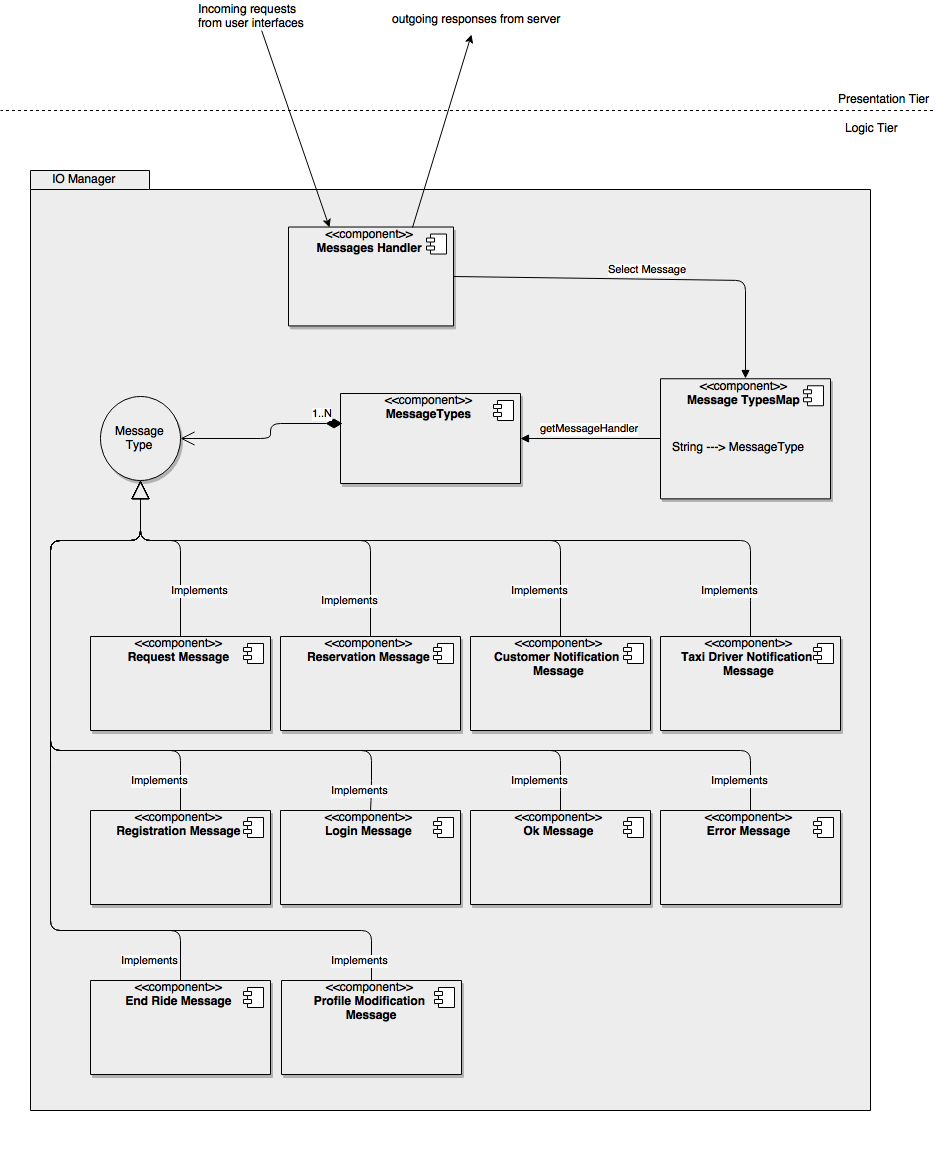
\includegraphics[width=\textwidth, scale=0.5]{../images/IOManager.png}
			\caption{IO Manager Structure}\label{fig:IOManager}
		\end{figure}
	
\end{document}